\section{\textbf{Parallel Automata Processor}}
In this section we discuss the proposed framework and architecture \cite{1} needed for effective parallelization of NFAs on the Automata Processor(AP).

\subsection{Range Guided INput Partitioning}
Enumerating from all states of an FSM will lead to exponential
computational complexity. Fortunately, many of these states are impossible start states for the particular input segment. The range of
an input symbol is defined as the union of the set of all reachable
states, considering transitions from all states in the FSM that have
a transition defined for that symbol. During actual execution, the
range of the last input symbol in a particular segment determines
accurately the subset of start states for the next segment. Any states
outside this range are impossible start states. The proposed parallelization framework \cite{1} partitions the input such that input segments
end at frequently occurring symbols with small ranges to take advantage of minimum range symbols. The symbol chosen for an FSM
is obtained by offline profiling. Frequently occurring symbols are
chosen to ensure that the size of input segments are roughly equal.

\subsection{Enumeration using Flows}
Ideally, one can activate all start states and execute all enumerations simultaneously on one copy of the FSM. We know this is possible
and correct, given that AP seamlessly implements any number of
simultaneous transitions in a given cycle, and there is no limit on the
number of start states that are activated. This seems like a perfect
solution, except that we lose all information about enumeration paths.
After processing the input segments we know what are the end states
for all enumeration paths, but there is no way of knowing which path
lead to which end states. Recall that after an input segment finishes
execution, it will inform the next input segment which enumeration
paths were the true paths and which paths were false paths. The next
input segment then must only use the results and end states of true
paths and discard false paths.
In a conventional processor, enumeration paths are executed on
SIMD threads and thread’s local variables keep track of the start state
of each path. In the AP, however there is no notion of local variables
or state tracking. The only way to implement state tracking is by
propagating the start state via the routing matrix. Routing matrix
currently just routes 1 bit per state element pair (which encodes
transition between two state elements) and is already known to be a
bottleneck in the system, both in determining the cycle time, and area
complexity (occupies $≈30\%$ of the chip) \cite{1}. Augmenting the routing
matrix with state information leads to exponential space complexity.
Which is something that ,most of the authors we are reviewing, are not looking for.\\
\cite{1} solution is to leverage  AP's flows to solve the above problem of tracking the start states of enumeration flows.\\
The state vector allows AP
to context switch between two independent executions much like the
register save/restore that allows tasks to context switch on traditional
CPU architectures \cite{12}. The output match events also encapsulate
a flow identifier.
In our architecture each enumeration path is mapped to an independent flow and time division multiplexed on the same half-core.
By association to a flow identifier, we can easily track the enumeration paths that belong to each flow. The host CPU keeps a flow table
which tracks which start states (or enumeration paths) are mapped
to which flows.

\subsection{Merging Flows}
The speedup which can be obtained from our parallelization techniques relies on two factors, the number of input segments executing
in parallel and the time taken to complete each input segment. In
general the speedup obtained is equal to number of input segments
divided by slowdown experienced by the slowest input segment.
Slowdown of an input segment is simply the time it takes when
compared to the time it would have taken had we known the exact
start states for that segment.
By utilizing flows we have maximized the number of input segments, however time division multiplexing of flows also slows down
processing of each input segment. Specifically the processing time
of each input segment is proportional to number of flows for that
segment. The range guided partitioning method significantly reduces
the number of enumeration paths and hence the number of flows
needed.

\subsection{Composition of Input Partitions}
Once the input segments finish, the final output results can be obtained by combining the results of true paths of each segment. The
host CPU reads the final state vector from the AP and then constructs a Boolean array indicating which flow has results for true
enumeration paths. This Boolean array is checked when reading the
results out of the output buffer. Each output buffer entry has few
bits indicating the flow identifier. Only results for the output buffer
entries which match with true flows are reported.

\subsection{Put it Together}
This section describes our overall framework for parallelizing NFAs
on the AP. Figure 4 [1] brings together all the concepts discussed in this
section to illustrate our overall framework. The parallelization framework consists of pre-processing steps and dynamic runtime steps.
First, the range is computed for all input symbols and a frequently
occurring symbol is chosen based on profiling (Section 3.1). This
is followed by the merging the states in the range table into flows
based on connected components and common parents.
This step generate the contents for the
State Vector Cache (SVC). The state vector cache is then loaded
onto the AP chips. This pre-processing can be augmented to the
compilation and configuration process for the AP. Following this,
the input is partitioned at boundaries of the chosen range symbol.
Each input segment starts getting processed in parallel on AP halfcores. Deactivation and convergence checks occur dynamically to
invalidate redundant or unproductive flows .
A segment can also receive a flow invalidation vector from the previous segment during its runtime. Once an input segment finishes, the
composition of output reports happens in the CPU 
\begin{figure}[!h]
    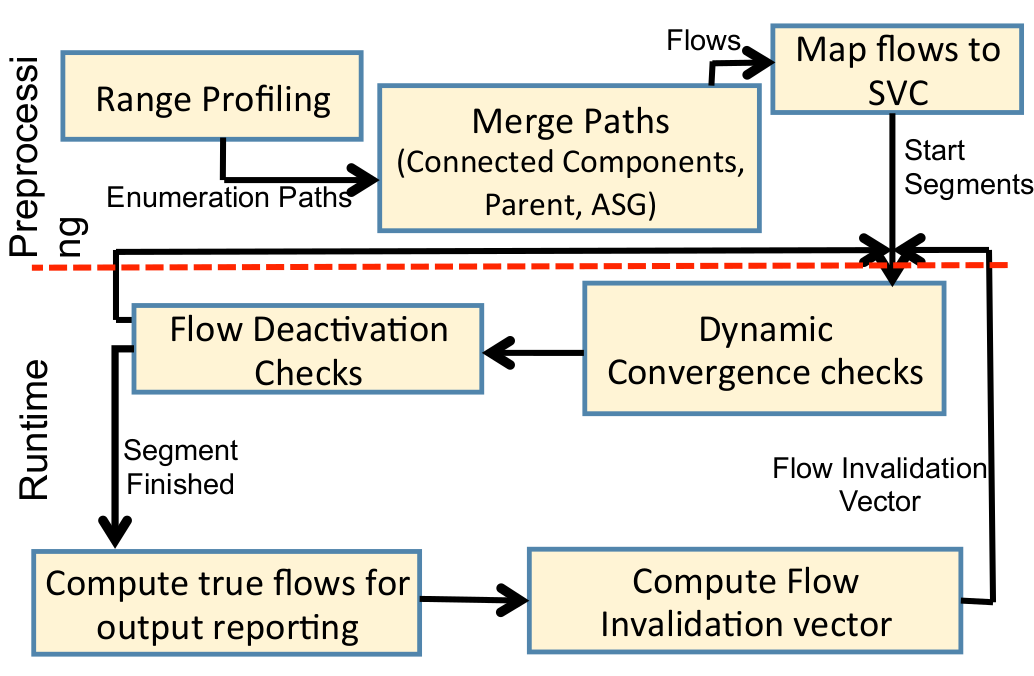
\includegraphics[width=\linewidth]{fx.png}
    \centering
    \caption{Overall framework.}
\end{figure}